\chapter{Method}
%\thispagestyle{empty}

\section{Framework}
To sparse code images and learn big dictionaries we design a software framework

\subsection{Signal representation}
\label{sec:signal_representation}
To be able efficiently sparse code images it is necessary to prepare the
image data. The signal preparation mainly consists of two sub steps.
\begin{itemize}
 \item Color space conversion
 \item Spartial saparation
\end{itemize}

\paragraph{Color space conversion} As we mainly use sets of natural color images
and graphics we require to work with multi-channel data. Commonly presented in
the three channel RGB color space.
When dealing with multi-channel data (e.g. RGB images) each channel can be coded
separate or as a concatenation of each signal into a single one. These
approaches can lead to color bleeding \cite{mairal08sparse} \Todo{add picture}
%Nevertheless 
A solution would be to add a constraint to the sparse coding that pays attention
the correlation of the channels. \Todo{add formula from paper} 
Fortunately this problem vanishes with big dictionaries and large training sets.
\cite{mairal08sparse}

%\paragraph{Chroma sub-sampling} is used to reduce the amount of data required
%by color information while preserving perceptual image quality. 
The human eye is good at sensing small difference in brightness but lacks the
ability exactly differentiate small changes in color. \emph{Chroma sub-sampling}
takes advantage of this human flaw. First the image gets converted into the
$YC_bC_r$ color space, which describes an image in a brightness/luminance (Y)
and two color/chroma components (Cb and Cr). Then the visual more relevant
brightness/luminance channel will be coded in the full resolution while the
color/chroma components can be sub-sampled with only minor loss in perceptual
quality. This procedure, illustrated in fig. \ref{fig:YCbCr}, is one key element
in lossy image compression. 
\begin{figure}[h]
\centering
%\includegraphics[scale = 0.25]{images/chroma_subsample.pdf}
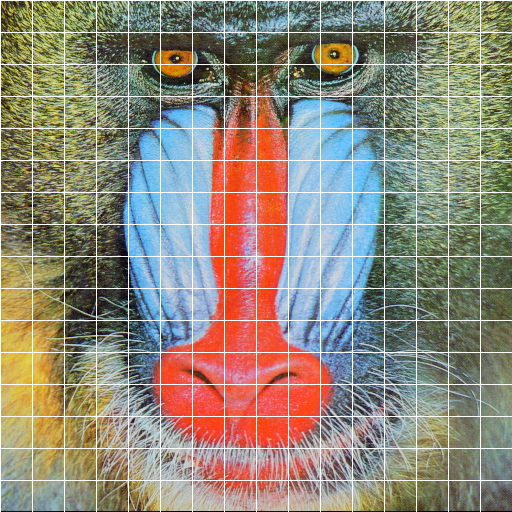
\includegraphics[scale = 0.25]{images/segmentation.png}
\label{fig:YCbCr}
\caption{RGB $\rightarrow$ YCbCr}
\end{figure}


\paragraph{Spartial seperation}
As the sparse coding process is operation on signal vectors it is required to
represent our 2-D image data in a set of 1-D vectors with size $m$. We extract
blocks of size $n \times n=m$ from the images. Typically dealing with block
sizes of $n=8,..,20$. The blocks get extracted in a raster either with
overlapping content or disjoint from each other. Figure\ref{separation}
illustrates this separation step.
\begin{figure}[h]
\centering
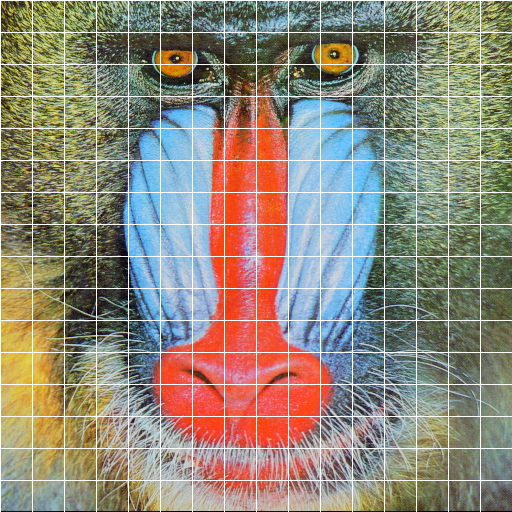
\includegraphics[scale = 0.25]{images/segmentation.png}
\caption{spatial separation}
\label{fig:separation}
\end{figure}

\subsection{Sparse coding step}
When coding a large number of small or medium sized decomposition problems,
which is the case for small image blocks in large image sets, some
optimizations can be made on the sparse coding algorithms. 
For the framework we chose batch modified versions of the OMP for $\ell_0$
regularization and the LARS-Lasso for $\ell_1$ regularization in the sparse
coding step to address this circumstance. 

\subsubsection{Batch-OMP}
In 2008 Rubinstein et al.\cite{Rubinstein2008} presented a speed improved
version of the orthogonal-matching-pursuit(\ref{sec:omp}) called
\emph{Batch-OMP}. The speed gain of \prettyref{alg:batchOMP} is achieved
by modifying the OMP in a way that can effectively sparse code
multiple signals in parallel. One key element of the optimizations is the
pre-computation of the gram matrix $G=D^TD$ which can efficiently be reused
for each signal. Another optimization to a single signal coding step itself
(\prettyref{alg:batchOMP}) is the cholesky factorization of $\left( D_A^T D_A
\right)^{-1}$ (line \ref{alg:OMP_DTD} of \prettyref{alg:mp}). $D_A^T
D_A$ is a symmetric and positive-definite matrix and can be cholesky decomposed
into $LL^T$. Even better, due to the nature of the algorithm composing $D_A$
by adding additional row and columns to it, $L$ can be build up during the
computation. This reduces the computational cost of the algorithm drastically.

\begin{algorithm}[H]
\caption{Parallel coding}
\label{alg:parallel}
\begin{algorithmic}[1]
\REQUIRE $X =[x_1,...,x_k]  \in \mathbb{R}^{m \times k}, D  =[d_1,...,d_p]  \in
\mathbb{R}^{m\times p}, \epsilon \in \mathbb{R}, \alpha =
[\alpha_1,...,\alpha_p] \in
\mathbb{R}^{p}$
\STATE pre-compute $G \gets D^TD$
%\STATE $\epsilon \gets X^TX$
\FOR {$i = 1$ to $k$}
\STATE Compute $\alpha_i$ using \prettyref{alg:batchOMP} or
\ref{alg:lars} for all ${x_i}$ in $X$
\ENDFOR
\RETURN $\alpha$
\end{algorithmic}
\end{algorithm}

\begin{algorithm}[H]
\caption{Batch-OMP}
\label{alg:batchOMP}
\begin{algorithmic}[1]
\REQUIRE $x \in \mathbb{R}^{m}, G  \in
\mathbb{R}^{m\times m}, \epsilon \in \mathbb{R}$
\STATE $A \gets \emptyset,\alpha \gets 0,\gamma \gets D^Tx,\delta^0 \gets
0, \epsilon^0\gets x^Tx,L\gets[1],n\gets1$
\WHILE {$ n<L$ \AND $\epsilon^{n-1} > \epsilon $}
\STATE $k \gets \argmax_k\lvert \alpha_k \rvert$
\IF {$n>1$}
\STATE $w \gets L^{-1}G_{A,k}$
\STATE
\begin{align}
L \gets \left[
\begin{array}{ccc}
L & 0\\
w^T & \sqrt{1-w^Tw}
\end{array}
\right]
\end{align}
\ENDIF
\STATE add variable to active set: $A \gets A \cup \{ k\}$
\STATE $\alpha_A \gets (L^T)^{-1}L^{-1}\gamma_A^0$
\STATE $\beta \gets G_A\alpha_A$
\STATE $\gamma \gets \gamma^0-\beta$
\STATE $\delta \gets \alpha_A^T\beta_A$
\STATE $\epsilon^n \gets \epsilon^{n-1} - \delta^n + \delta^{n-1}$
\STATE $n \gets n+1$
\ENDWHILE
\RETURN $\alpha$
\end{algorithmic}
\end{algorithm}


%\subsubsection*{Optimizations}
%\Todo{remove?}
All modification lead to significant speed increase when coding large sets of
signals. While $L$ is very small the main factor of the computation is
the multiplication of $D$ with a vector. Detailed information on the complexity
and speed gain can be found in the corresponding paper on the
Batch-OMP\cite{Rubinstein2008}. 

% with a complexity of $O(mp)$. 
%This modification reduces the complexity of the OMP from $O\left(L2mp + 2L^2m +
%2L(p+m) + L^3\right)$ to $O\left(2mp + L^2p + 3Lp + L^3\right)$ 
%with pre-computation $\left(mp^2\right)$ as shown in\cite{Rubinstein2008}. 

%more signals than dictionary elements.

\paragraph{LARS-Lasso} is chosen as it one of the fastest $\ell_1$
regularizationand and it leads to good results for signals of low dimension and
with high correlation of dictionary elements. Both conditions are satisfied
when coding small image blocks.

The same pre-computation of the gram matrix used in the Batch-OMP can also
be applied to the LARS-Lasso algorithm. The framework uses a simple combination
of parallel coding\ref{alg:parallel} and the LARS\ref{alg:lars} presented
in\ref{sec:lars}.

\subsection{Learning step}
The majority of learning experiments in literature were made on
samples of sliding blocks from single images or small sets of images.
A good strategy when the learned dictionaries are only used for operations on
those images. The dictionary atoms learned from those image have a high
correlation to the image content.  When looking at large sets of images and many
different blocks we start to talk about a different game. Now each dictionary
elements dends to captures more general structurs of the signals.

For the learning step we use the \trainDL learning algorithm. As an on-line
learning algorithm it is able to learn dictionaries from very large sets of
training data.

Section \ref{sec:signal_representation} already describes that the learning
process is not limited to gray-scale oder RGB image signals. The presented
algorithm can be applied to different kinds of signals. Such as images in other
color spaces, low/high pass filtered sub-images or signals from another domain
like audio or text. 


\subsubsection{Initialization}
At the start of a training process it is requires to initial the
dictionary with start data. Otherwise the sparse coding step will only find
trivial solutions with all coefficient being zero. Which then will have no
effect in the learning process.

There are two common ways to initialize the dictionary using random data or
selecting random elements from the training data. The framework supports 
both ways of dictionary initialization. \Todo{optional: image}
%can be tested and the quality will be compared.

\subsubsection{Convegence}

Depended on block size, dict size, average nuber of coefficients.
Block size of the atoms
Coefficients per signal code respectively $\lambda$
Dictionary size 
Most of the experiments in on small sets of 
See the differences in the selection sceme.
In the beginning OMP is very random.


\subsubsection{Clustering}
One reason not to learn big dictionaries in a single step is the fact that
learning such big dictionaries leads to huge memory consumption and coding time.
To address these problems we investiage strategies to distribute the workload of
the learning step onto multiple clients with a clustering approach similar to
MapReduce. 

One strategy would be to utilize the batch\ref{sec:trainBatchOptimize}
modification of the LARS-Lasso algorithm. Rather than just coding a small batch
of signals in one itereation of the traning step\ref{alg:trainDL} we code one
batch on each client of the cluster and merge all of them before
applying\ref{alg:update}. Keeping the dictionary in each iteration fixed
for every batch coding client. The problem is that it is still required 

Another strategy is to learn several smaller dictionaries on disjoint sets of
training data and when the learning step ended, merge the dictionaries
into a bigger one. The merge process starts with an empty dictionary and
sucesifly adds atoms from the dictionaries of the learning step to the
new dictionary unless the atom can be reconstructed with few atoms of the
current state of the new dictionary. The drawback of this approach is fact that 
each atom will be less corelated to whole training set.

\begin{algorithm}[H]
\caption{Merging dictionaries}
\label{alg:merging}
\begin{algorithmic}[1]
\REQUIRE $ S = (D_1,...,D_k) \text{ set of dictionaries } D \in
\mathbb{R}^{m\times p}$

\STATE $D_{new} \gets D_{1}[1], n \gets 0$
\FOR {$i = 1$ to $k$}
\FOR {$j = 1$ to $p$}
\STATE sparse code 
\STATE $n \gets n+1$
\ENDFOR
\ENDFOR
\RETURN $D$
\end{algorithmic}
\end{algorithm}

Taking strategy two even futher is to learn smaller dictionaries from different
sets of images or charakteristics. Such as paintings, gray-scale sketches and
smooth images animation. For example learning dictionaries for very specific
classes of images can be utilized for classification tasks. Somthing that can
come in handy when applying it to operations like search in large image
databases.

%\paragraph{1. one dictionary per client}
% -> merge
% -> drawback: less idipendent learning
%\paragraph{2. one chunk of sample per client}
%  -> merge after evey train iteration
% drawback: many samples per train step

\subsection{Application to image compression}
Experiment on sparse coding as a tool for compression have been done
before\cite{Lewicki1999,?} but mainly in theory with generated bases
dictionaries for comparison and approximations on entropy and resulting
bits-per-pixel. Leading to better density with learned dictionaries over
designed. 

Todays lossy image compression algorithms are primary based on scientific
findings about visual perception reaching far back in the 1970s\cite{?} and
good entropy encoding of the data. Both elements led to to the
following main steps in lossy image compression algorithms:
\begin{itemize}
 \item lossy color space conversion
 \item sub-sampling amd spatial separation
 \item coding of image signals
 \item quantization to reduce of the number of non-zero coefficient 
 \item lossless entropy coding of the coefficient 
\end{itemize}
We already describe the first two steps in
section\ref{sec:signal_representation}. So we will concentrate on the last
three.
%As learned dictionary elements show also locality in time like , 
%But real practical application is an open question
We add quantization and entropy encoding after the sparse coding step to develop
a simple real world compression algorithm for sparse coded images.


\paragraph{Signal coding}
The actual coding step of the prepared signals is a simple application of one
of the sparse coding algorithms we present in\ref{chap:sparse_coding}.

%But before we can actually code signals we need a good dictionary.
%We learn dictionaries from our training sets  block sizes Number of
coefficients

\paragraph{Quantization}
The idea of quantization is that the human eye is not good at seeing high
frequency brightness variations.

quantized coefficient. Additional zero coefficients from the quantization step
are removed.

Fixed quantization or learned from dictionary

%The JPEG algorithm 
We adopt the idea of visual perception idea of JPEG to our
approach and sort our element by their frequencies.
The random distribution of the atoms in the dictionary 
We concentrated on two fixed quantization factor and the analysis of the
dictionary elements.

%copy
%The human eye is good at seeing small differences in brightness over a
%relatively large area, but not so good at distinguishing the exact strength of
%a high frequency brightness variation. This allows one to greatly reduce the
%amount of information in the high frequency components. 
%Copy
%The human eye is good at seeing small differences in brightness over
%a relatively large area, but not so good at distinguishing the exact strength
%of a high frequency brightness variation. This allows one to greatly reduce the
%amount of information in the high frequency components. This is done by simply
%dividing each component in the frequency domain by a constant for that
%component, and then rounding to the nearest integer. This rounding operation is
%the only lossy operation in the whole process if the DCT computation is
%performed with sufficiently high precision. As a result of this, it is
%typically the case that many of the higher frequency components are rounded to
%zero, and many of the rest become small positive or negative numbers, which
%take many fewer bits to represent.





\begin{figure}[h]
\centering

\includegraphics[width = 0.75\textwidth]{images/sorted.png}
\caption{sorted learned dictionary}
\label{fig:sorted}
\end{figure}

\paragraph{Data encoding}
%The sparse vector for every are encoded in 2 bytes index and a single byte
Coefficients
Indices
In 1999 Lewicki et al.\cite{Lewicki1999} already made some on comparison 
the bpp required for encoding of the sparse matrix data. Besides the estimation
of the compression we also really applied some coding schemes to compare real
world compression data.
\cite{Murray2006}

\begin{description}
 \item[Run-length encoding (RLE)] The main requirement to work well is
that the data consists of larger groups of the same data.
  \item[Huffman coding] Elements that occur often are encoded with less bits.
Leading to a table and a block of encoded data.
  \item[Arithmetic coding] is ...
While arithmetic coding often yields better compression results than Huffman
coding. The higher processing requirements for coding and the current patent
situation makes the algorithm unpopular for coding compared to the archived
compression benefit.
\end{description}

We apply RLE to the sparse matrices and then huffman coding to the remaining
data.
%The sparse vector for every are encoded in 2 bytes index and a single byte 
%quantized coefficient. Additional zero coefficients from the quantization step
%are removed.

As mentioned in in \ref{sec:headers} we are aware of the fact that besides
the actual sparse matrix data we also have other file informations and meta
data but ignore them for simplification.
  
\subsection{Implementation}
%\subsection*{Software}
The sofware framework consists of a library for sparse coding image signals 
and learning dictionaries, a command line interface to the library and
miscellaneous scripts for distribution of coding and learning jobs and
some a test suite.

The whole sparse coding and training library is written in C++ with
additional use of the OpenCV, Eigen and OpenMP libs. All operations use double
precision. 

Eigen\footnote{\url{http://eigen.tuxfamily.org/}\cite{Eigen}}
is a template library for fast vector and matrix operations 
and includes some linear algebra algorithms. It is mainly used for operations on
dense and sparse matrices and solving of linear equation
systems. 

OpenCV\footnote{\url{http://opencv.willowgarage.com/}\cite{OpenCV}} as
in \emph{Open Computer Vision Library} is mainly used for
image read and write operations, color space conversion adn DCT for the
quantization matrix generation step. 

OpenMP \footnote{\url{http://www.openmp.org/}\cite{OpenMP}} is a preprocessor
based application programming interface (API) for C,C++ and Fortran that enables
the user to distribute code block and loops to multiple CPU cores. In situations
where it is applicable OpenMP is used to utilize multi-core CPUs. 

\Todo{add diagram}
Split image into sub images, convert sub image to samples from image blocks, 
train dict with samples or just code samples - save dictionary/image
Image block size, block selection strategy can be specified.

\paragraph{Coding}
The sparse coding step can be configured to use either the Batch-OMP and 
set a limitation to the maximum number of coefficients or the LARS-Lasso 
and set the regularization(\ref{eq:l1}) factor $\lambda$.
The Batch-OMP implementation is based on the implementation
of \cite{Rubinstein} OMPBox with technical modifications to fit into our
framework. The LARS-Lasso C++ implementation is based on the Matlab
implementation of\cite{Strand2005} and the original
paper\cite{Efron2004} on the algorithm.

\paragraph{Learning}
The \trainDL is a straight forward C++ implementation of the
learning algorithm presented in\cite{Mairal2010}. It is an implementation of the
basic version of the algorithm with the batch optimization applied. Batch-OMP
and the LARS-Lasso coding method can be utilized for the coding part.
Dictionary size and the number training signals for each iteration can be
speficied.


\paragraph{Command line interface}
%\lstinputlisting[language=C++,caption=Training]{listings/test.cpp}

\paragraph{Miscellaneous}
Besides the actual coding software some other tools for
additional tasks were used. Several bash and ruby scripts for workload
distribution onto the clients, aggregation and evaluation of the results.
Also he ImageMagick\footnote{\url{http://www.imagemagick.org/}} toolkit was used
for image conversion into JPEG and JPEG 2000 and for some image comparison
tasks.


\section{Experiments}

%\Todo{move to results? or at end of method}
\subsection{Comparison terms}
Before we go further and present the experiments and their results  it is
necessary to introduce some additional terms. Such as metrics to measure
their performance.

\paragraph{Mean squared error (MSE)} is an error measurement that
describes the error/noise between an given or measured reference signal $x$
and  and the reconstruction(noisy approximation) $\tilde{x}$ of it.
Mathematically it is defined as the average of the squared error between two
signals.
%The mean squared error is defined as:
\begin{align}
 MSE = \frac{1}{n} \sum_{i=0}^{n} \left( {\lVert x_i -
\tilde{x}_i\rVert^{2}}\right)
\end{align}
We primarily use it for testing dictionary learning convergence and as a
sub term for the measurement described in the next paragraph.

\paragraph{Peak signal-to-noise ration (PSNR)} describes the ratio between the
error/noise affecting a signal/reconstruction and the maximum possible signal
amplitude. It is expressed in a logarithmic decibel scale.
\begin{align}
 PSNR = 20 \cdot \log_{10} \left(\frac{MAX}{\sqrt{MSE}}\right)
\end{align}
Where $MAX$ is the maximum possible value of our signal. For an 8-bit
image it would be 255. For a 32-bit normalized image it would be 1. And $MSE$ is
the mean squared error between a reference signal and its reconstruction. The
PSNR is undefined for zero noise.

The PSNR is primarily used for comparison of the reconstruction quality of
lossy compression algorithms. Typical values for a lossy reconstruction lie in
a range between 30dB and
50dB.\footnote{\url{http://en.wikipedia.org/wiki/Peak_signal-to-noise_ratio}}
%e.g. relevant for de-noise

\paragraph{Bits per pixel (bpp)} 
For the comparison of compression ratio of images another well known practice is
to measure the required \emph{bits per pixel} short bpp. The bbp are calculated
by dividing the raw image data by the image's dimensions. For example an
uncompressed RGB color image with 8-bit of color depth requires 24-bits per
pixel, respectively a gray scale image with 8-bit for a single channel requires
8-bits. While compression algorithms are able to encode multiple pixels with few
coefficient leading to much lower bpp rates.
Looking at other well known compression algorithms such as JPEG or
JPEG 2000 a common ratio is about $\sim1.8$ bits-per-pixel for average
quality compression( JPEG quality of 50) of an natural image. 
\Todo{example image?, lower bit rates, Lewicki estimate for sparse coding}

Besides the raw pixel data, images formats usually contain a certain amount
of extra data from file headers and meta data. Fortunately we can ignore this
for simplification as it is only a few bytes and not being actual pixel data.

\paragraph{Test data}
In addition to the introduced metrics it is common practice to use some image
sets to compare test results of the different algorithms and parameter
configurations. As the dictionaries are specificaly trained for
reconstruction of the data in the training sets it is mandatory to also use
these image to test the reconstruction and compression quality.
\begin{figure}[h]
\centering
\subfloat{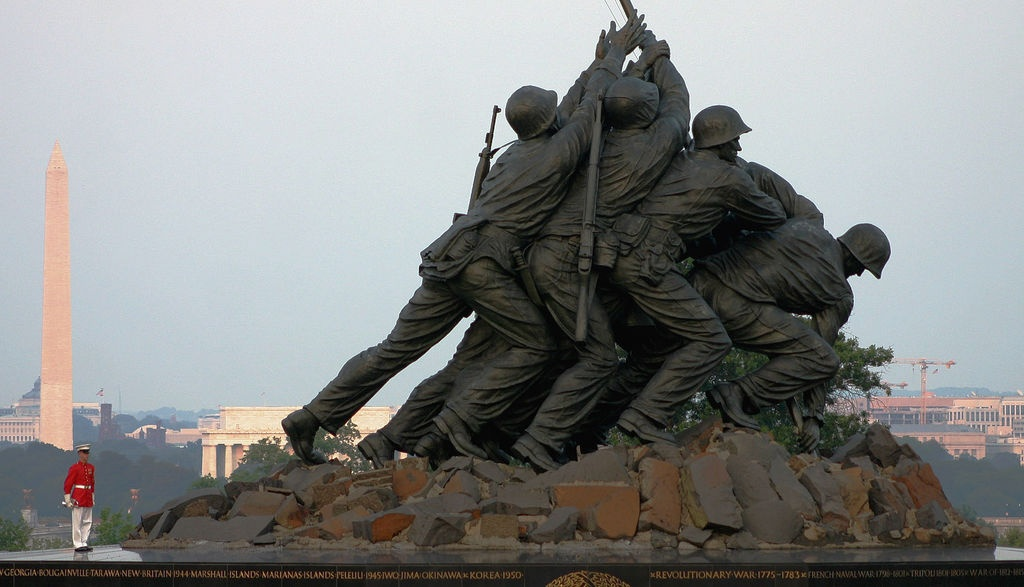
\includegraphics[width = 0.3\textwidth]{images/28979823.jpg}}
\hspace{5mm}
\subfloat{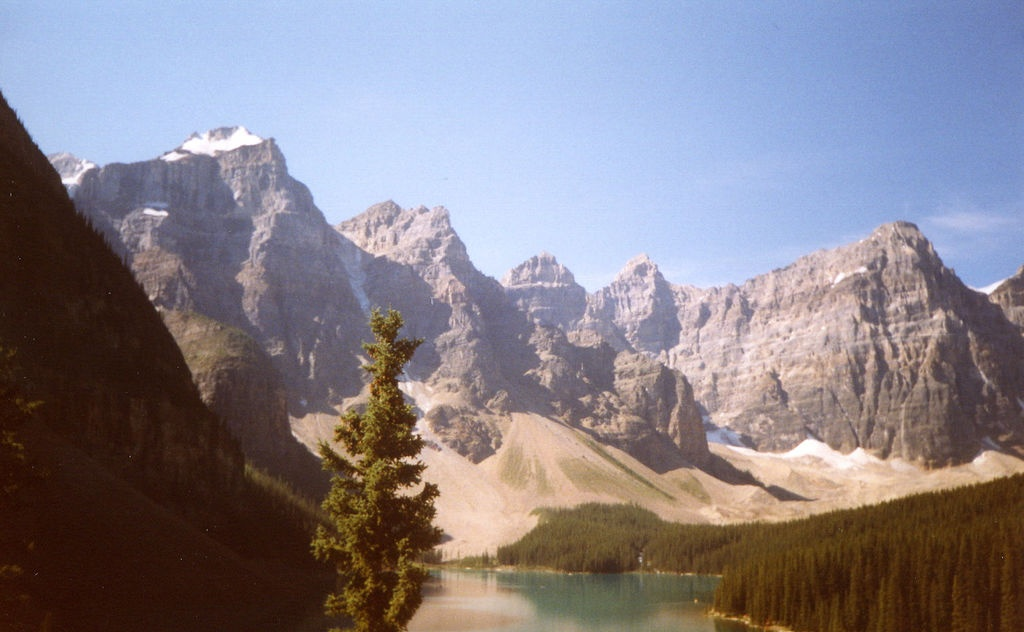
\includegraphics[width = 0.3\textwidth]{images/29018694.jpg}}
\hspace{5mm}
\subfloat{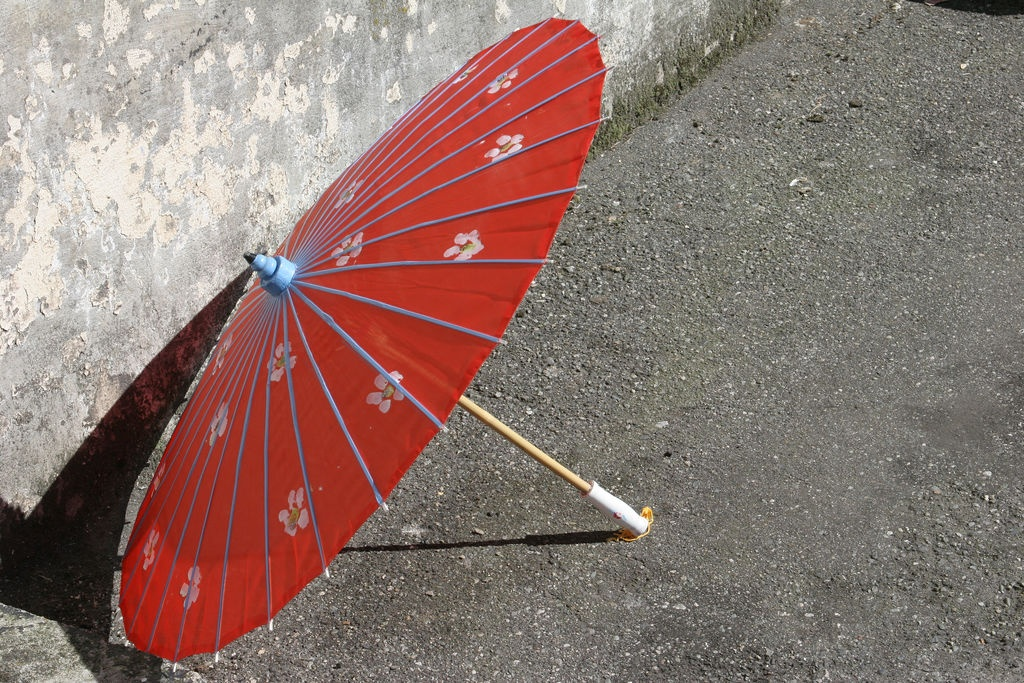
\includegraphics[width = 0.3\textwidth]{images/28874882.jpg}}
\hspace{5mm}
%\subfloat{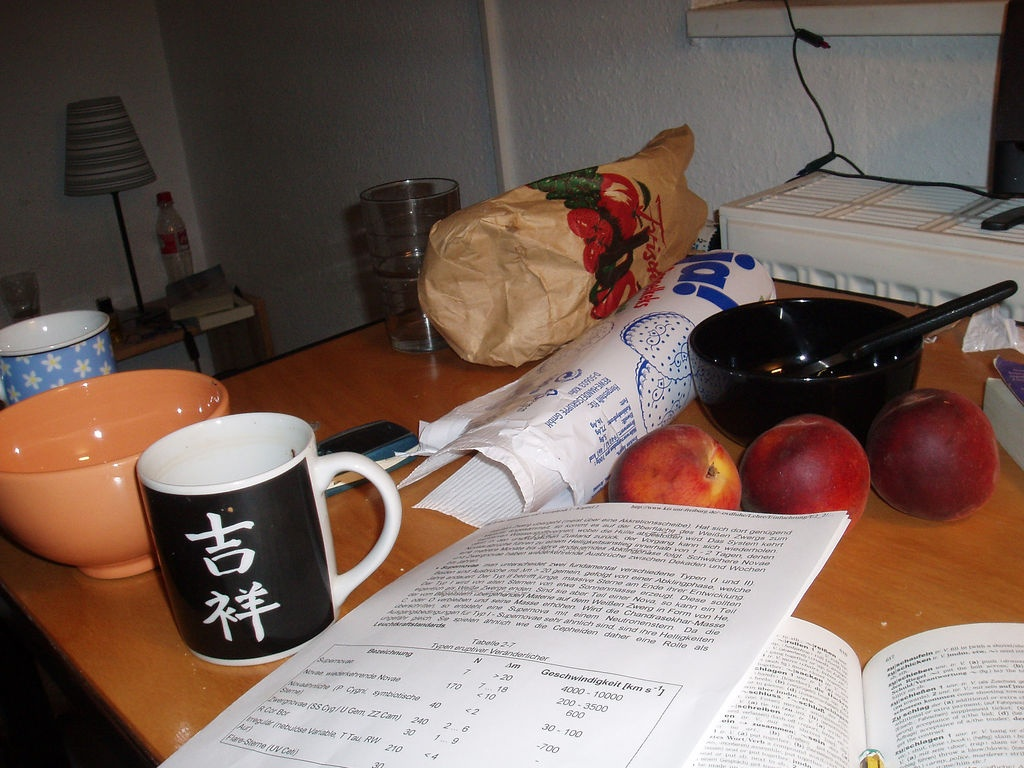
\includegraphics[width = 0.3\textwidth]{images/28848380.jpg}}
%\hspace{5mm}
%\subfloat{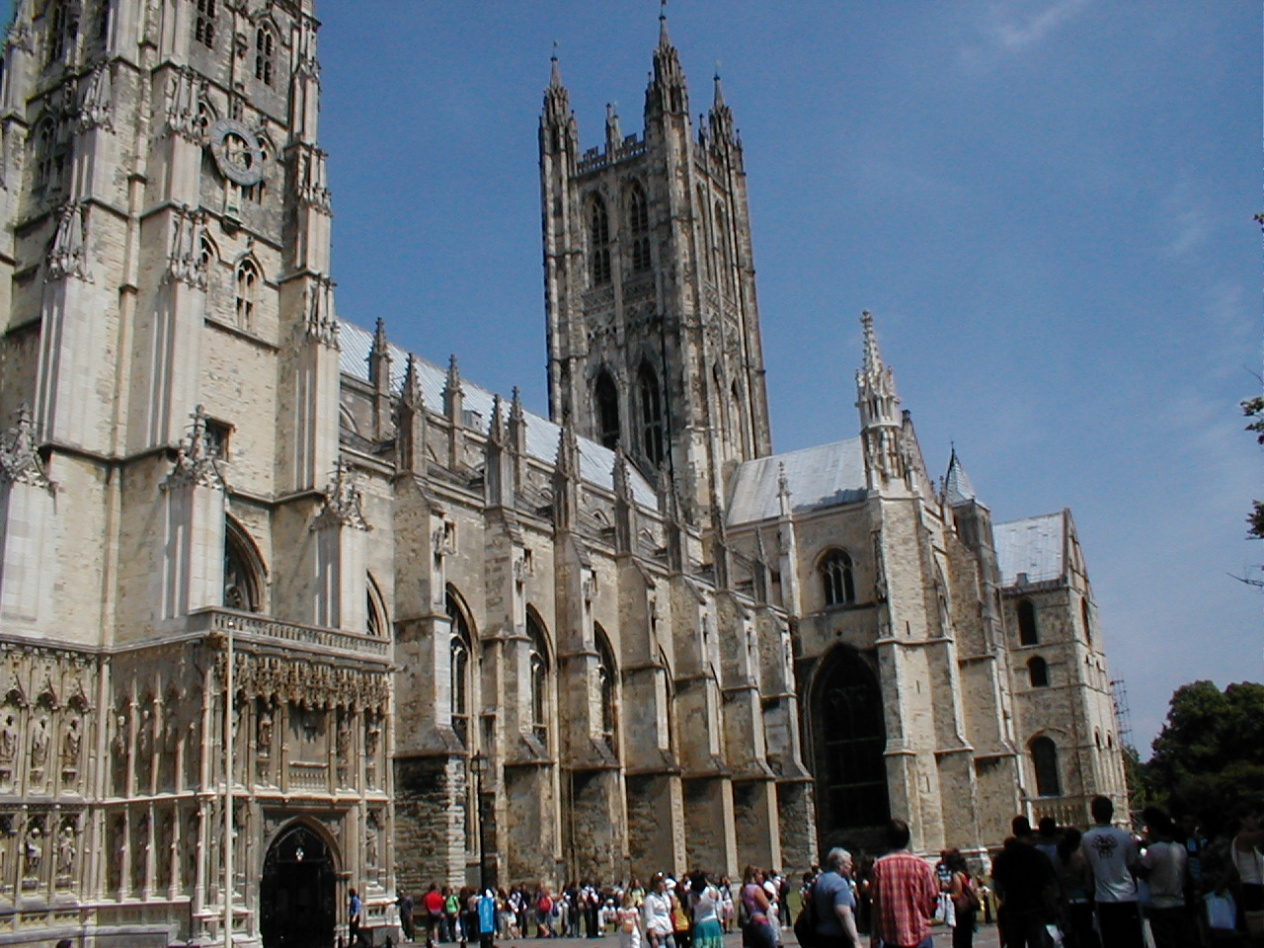
\includegraphics[width = 0.3\textwidth]{images/28859439.jpg}}
%\hspace{5mm}
\subfloat{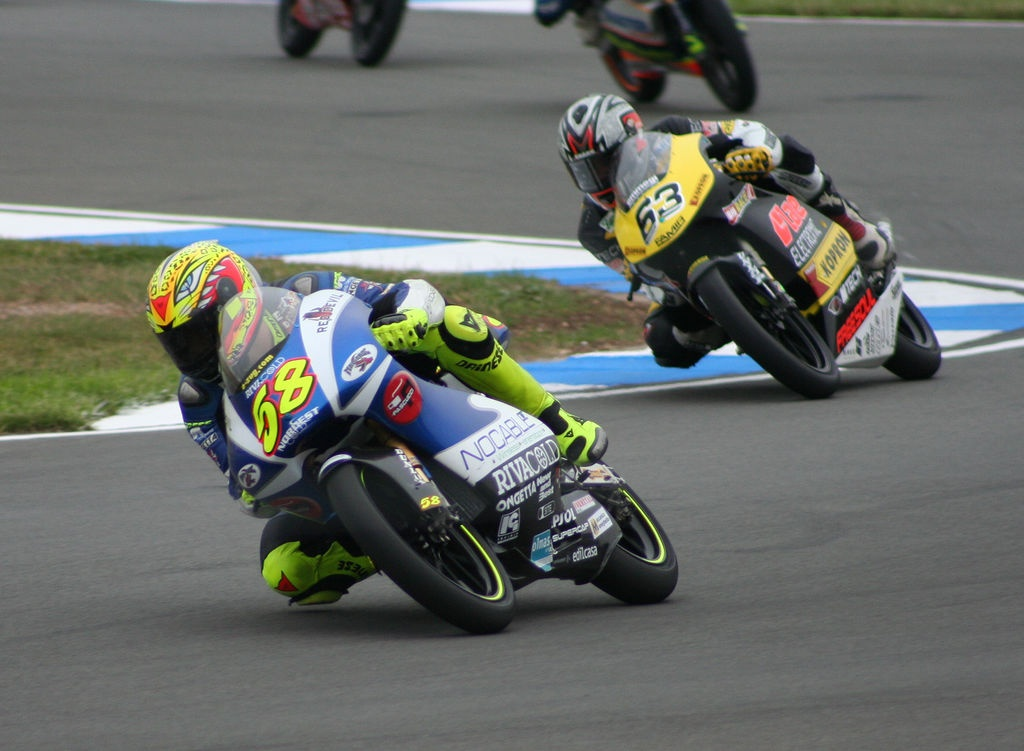
\includegraphics[width = 0.3\textwidth]{images/28803842.jpg}}
\hspace{5mm}
\subfloat{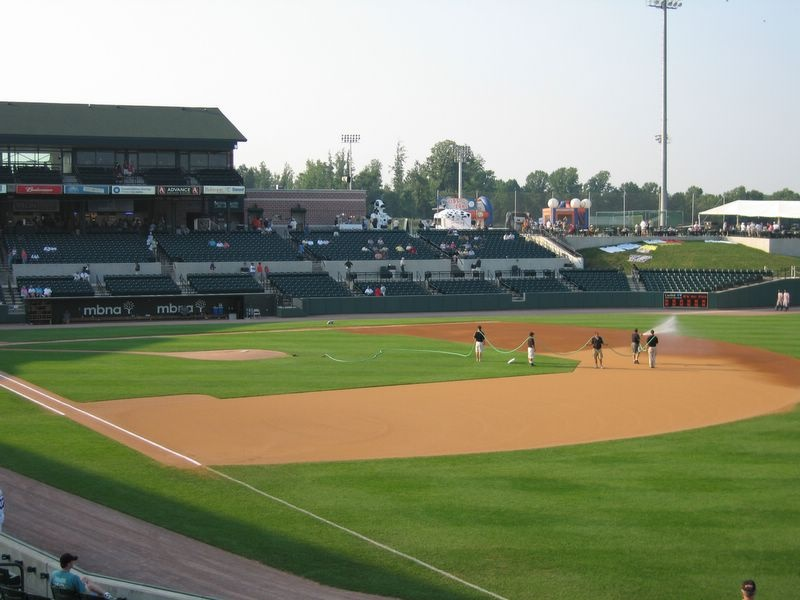
\includegraphics[width = 0.3\textwidth]{images/28894495.jpg}}
\hspace{5mm}
\subfloat{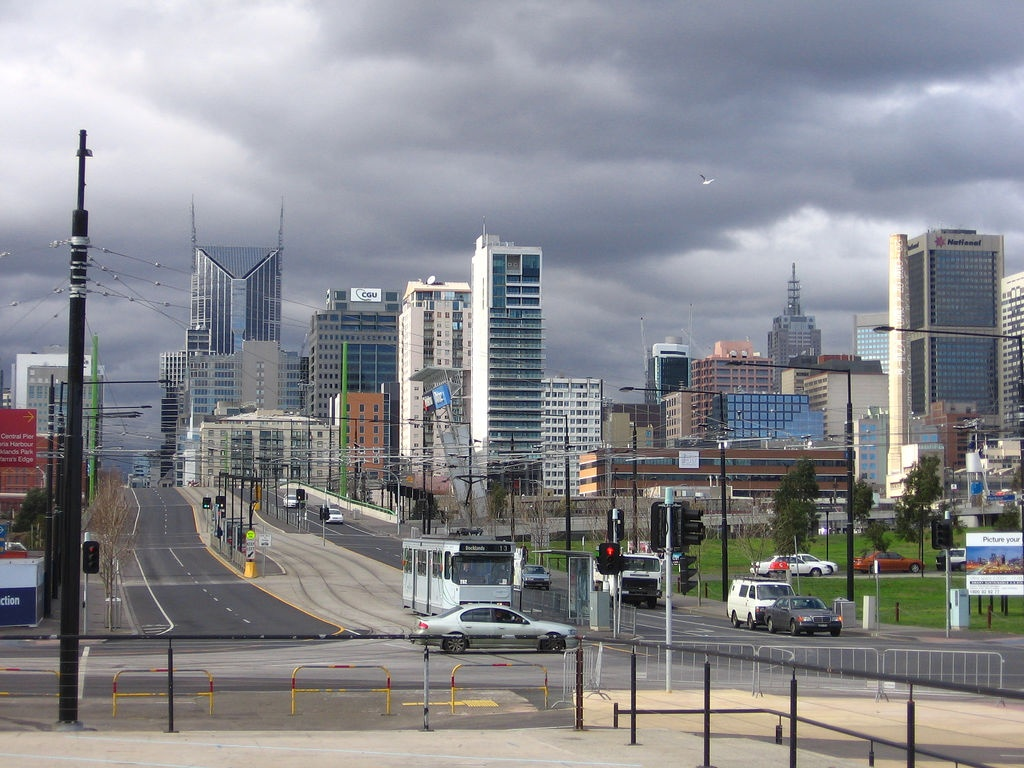
\includegraphics[width = 0.3\textwidth]{images/28952841.jpg}}
\caption{image from training set}
\label{fig:USC-SIPI}
\end{figure}
In addition to this we want to know how good the dictionaries can reconstruct
and compress images outside of the training set. For those comparisons we use a
well known set of standard test images from the \emph{USC-SIPI Image
Database}\footnote{\url{http://sipi.usc.edu/database/}}. They are often
used in image processing for evaluation of compression algorithms. 
Including pictures such as Lena, Mandrill and Peppers.
\begin{figure}[h]
\centering
\subfloat{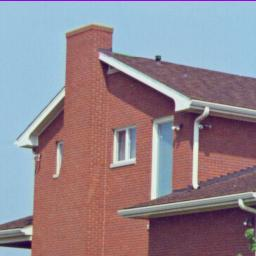
\includegraphics[width = 0.3\textwidth]{images/4_1_05.jpg}}
\hspace{5mm}
\subfloat{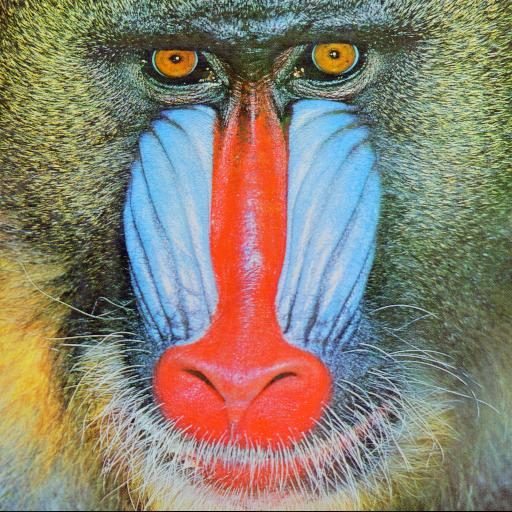
\includegraphics[width = 0.3\textwidth]{images/4_2_03.jpg}}
\hspace{5mm}
\subfloat{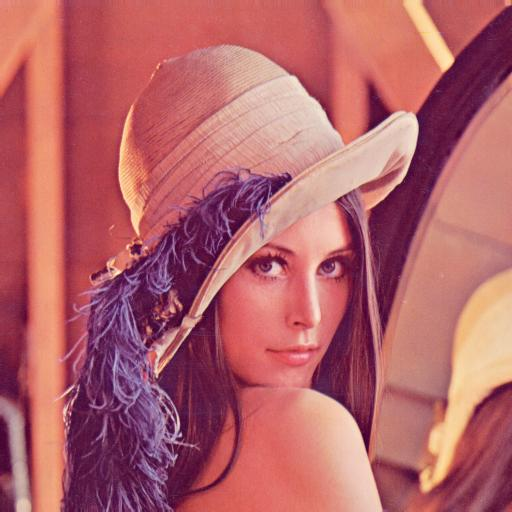
\includegraphics[width = 0.3\textwidth]{images/4_2_04.jpg}}
\hspace{5mm}
\subfloat{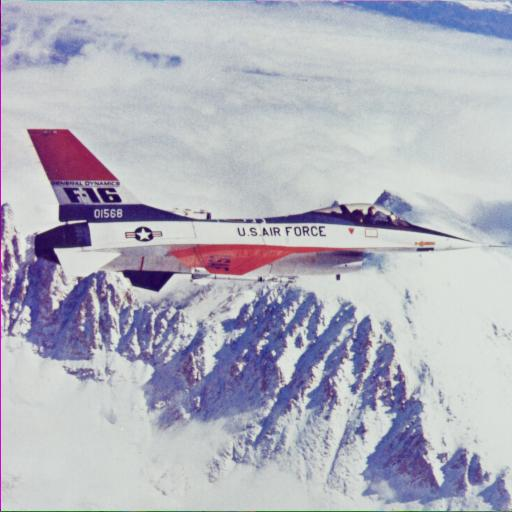
\includegraphics[width = 0.3\textwidth]{images/4_2_05.jpg}}
\hspace{5mm}
\subfloat{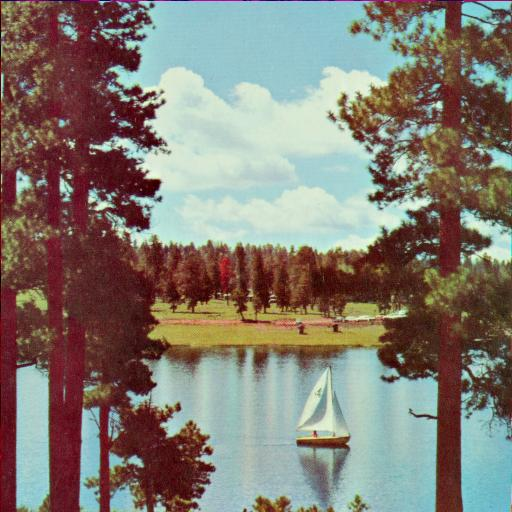
\includegraphics[width = 0.3\textwidth]{images/4_2_06.jpg}}
\hspace{5mm}
\subfloat{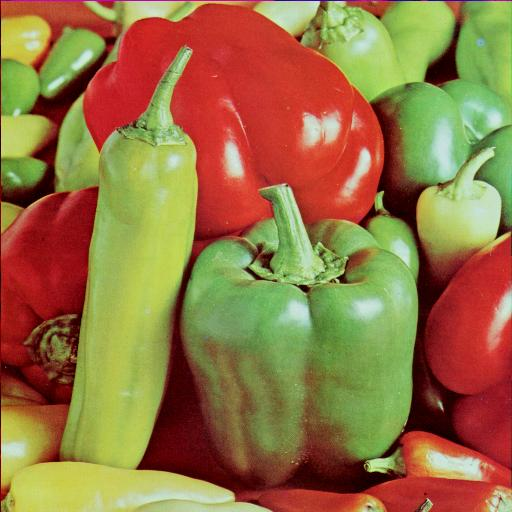
\includegraphics[width = 0.3\textwidth]{images/4_2_07.jpg}}
\caption{images from USC-SIPI Image Database}
\label{fig:USC-SIPI}
\end{figure}

\subsection{Training sets}
%\subsection{Learning specific dictionaries}
Section \ref{sec:learnForTheTask} mentions that one of the key
elements of the learning algorithms is the learning of specialization
dictionaries. Task specific training data is a common way to solve the problem
of finding  the right dictionary. Here learning for the task comes into
account. Such as de-noising/in-painting dictionaries directly learned from the
initial signal that gets de-noised or restored from in-painting. If the task
gets bigger it sounds logical to increase the size of training data and take a
bigger variety of signals to learn from.  We have a closer look at differences
of learned elements from specific sets of images. These sets include sketches,
still images of animations from Disney and post-impressionistic images from
Vincent van Gogh.  

Are big image collections specific enough to benefit from sparse coding?
%\thispagestyle{empty}

%\section{Experiments}
Comparission of the quality of dictionaries learnd via cluster strategy and
with normal single maschine were made.

\subsection{Hardware setup}
%Problems
%Big matrices
%Speed 
%Compression
%The 
Computations were made on Apple MacPro with ... \Todo{mac config}
and a cluster consisting of 100 nodes with each AMD Athlon X2 \Todo{athlon
config} running Debian 32-bit. Each client in the cluster calculated batches of
100 till 10,000 images based on the size of the training sets.

\subsection{Dictionary size}

\begin{table}[h]
\caption{dictionary size}
\centering
\begin{tabular}{l  c  c  c  c  c}
\toprule
Image & 1 & 2 & 3 & 4 & 5 \\
\hline
300 & 30 & 30 & 30 & 30 & 30 \\
600 & 30 & 30 & 30 & 30 & 30 \\
900 & 30 & 30 & 30 & 30 & 30 \\
1800 & 30 & 30 & 30 & 30 & 30 \\
3000 & 30 & 30 & 30 & 30 & 30 \\
\bottomrule
\end{tabular}
\end{table}

\Todo{small image sample comparision}
\begin{figure}[h]
\centering
\subfloat{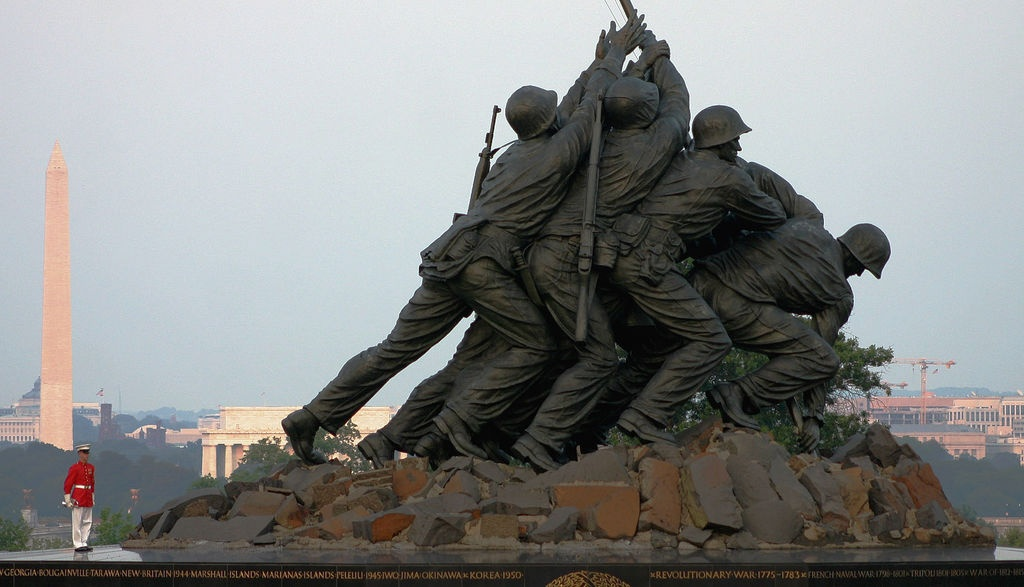
\includegraphics[width = 0.3\textwidth]{images/28979823.jpg}}
\hspace{5mm}
\subfloat{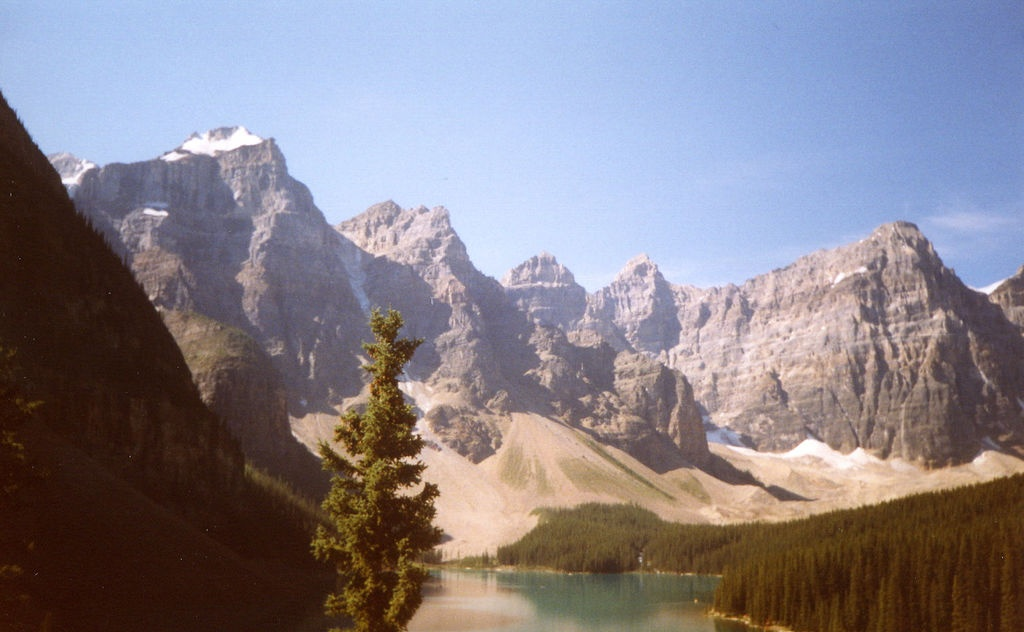
\includegraphics[width = 0.3\textwidth]{images/29018694.jpg}}
\caption{dict size difference}
\label{fig:dict size}
\end{figure}


Convergence


Mostly reduced to line segments and curve elements.
\Todo{Reconstruction results}
\subsection{Dictionary elements}
\begin{figure}[h]
\centering
\subfloat{
\includegraphics[width = 0.3\textwidth]{images/gradient.png}}
\hspace{5mm}
\subfloat{
\includegraphics[width = 0.3\textwidth]{images/checkerboard.png}}
\hspace{5mm}
\subfloat{
\includegraphics[width = 0.3\textwidth]{images/spot.png}}
\hspace{5mm}
\subfloat{
\includegraphics[width = 0.3\textwidth]{images/edges.png}}
\hspace{5mm}
\subfloat{
\includegraphics[width = 0.3\textwidth]{images/wavelet.png}}
\caption{image from database}
\label{fig:USC-SIPI}
\end{figure}

Learn basis similar to DCT and wavelets/bandelets(time and freq locality) with
increasing block size.
Similar to natural images.
compression dicts

% \begin{figure}[h]
% \centering
% 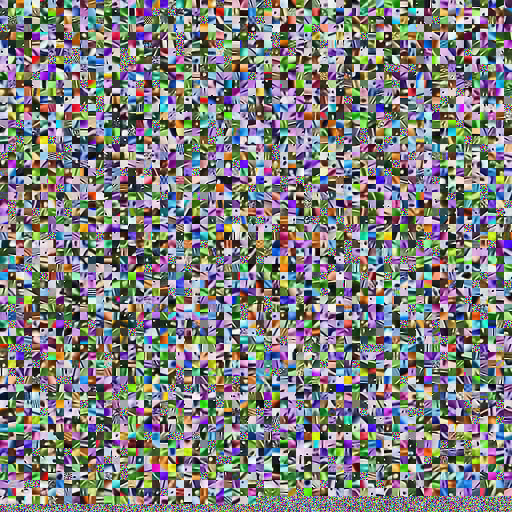
\includegraphics[width = 0.44\textwidth]{images/8_4000_10000_10_lasso.png} 
% \caption{8x8 OMP after some iterations}
% \label{fig:8_4000_lasso}
% \end{figure}
% 
% \begin{figure}[h]
% \centering
% 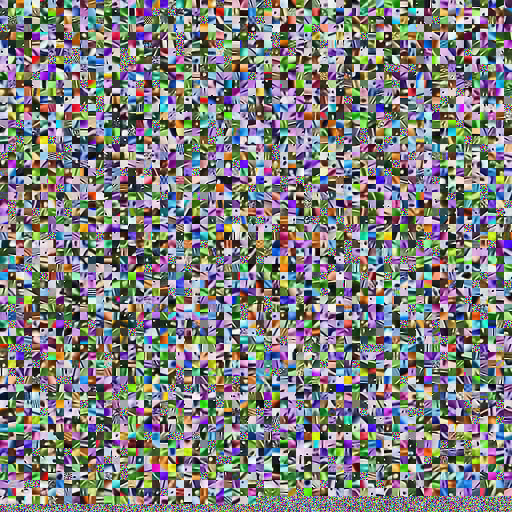
\includegraphics[width = 0.44\textwidth]{images/8_4000_10000_10_lasso.png} 
% \caption{8x8 LARS after some iterations}
% \label{fig:8_4000_lasso}
% \end{figure}

